\documentclass[uplatex,dvipdfmx,nomag,a4paper,oneside,onecolumn,12pt]{bxjsreport} % Japanese
%\documentclass[uplatex,dvipdfmx,nomag,a4paper,oneside,onecolumn,12pt, english]{bxjsreport} % English

\setpagelayout*{
    top=24mm,
    bottom=24mm,
    left=24mm,
    right=24mm,
    footskip=\heightof{/}*4,
}

\usepackage{preamble}

\usepackage{subfigure}
\usepackage{cite}

\usepackage[utf8]{inputenc}
\usepackage[T1]{fontenc}
\usepackage{lmodern}
\usepackage{newtxtext}
\usepackage{bm}

\usepackage{lipsum} % ダミーテキスト
\usepackage{layout} % レイアウト確認
\usepackage{pdfpages} % 表紙PDF挿入

\begin{document}

% \layout % レイアウト確認

%% 別PDFファイルを表紙として挿入する場合

%% 卒業論文
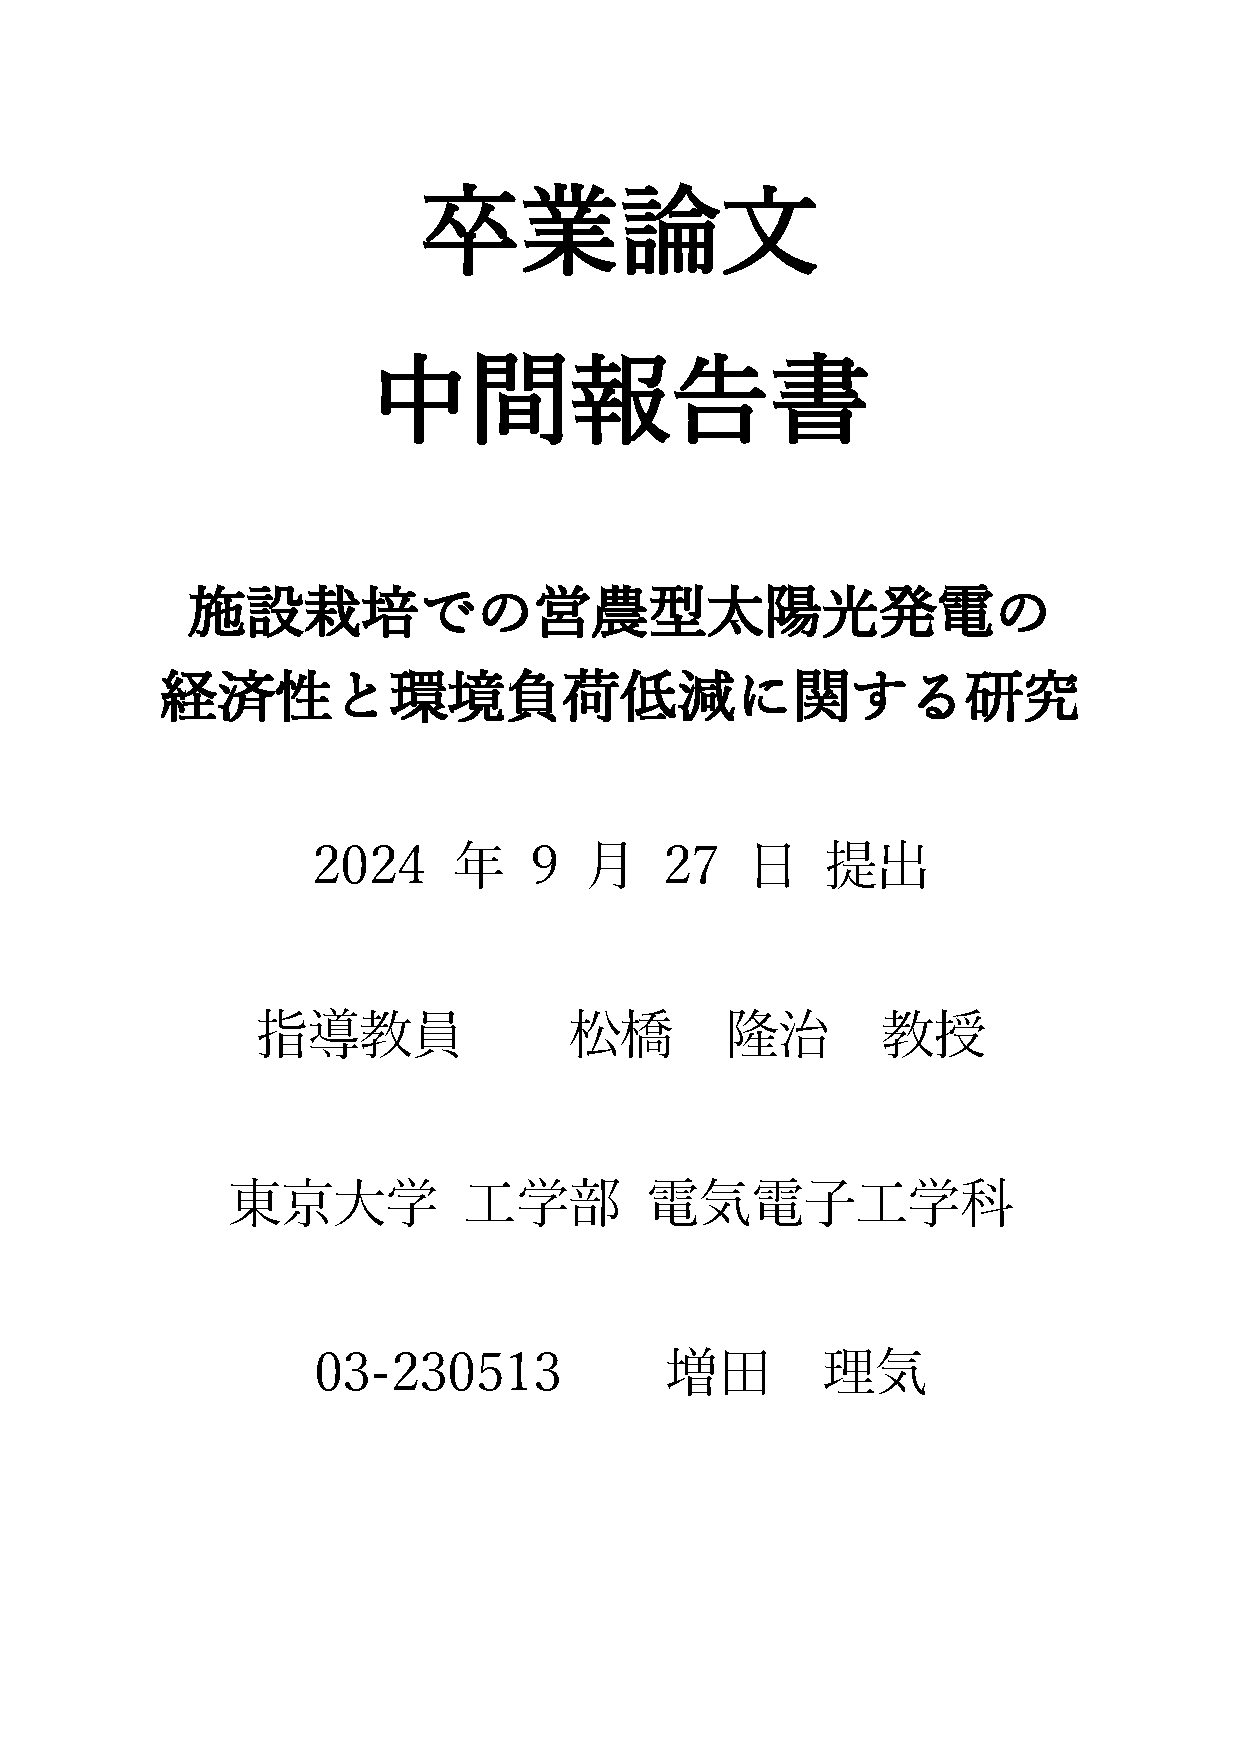
\includepdf{frontpage.pdf}

\frontmatter

\tableofcontents 

\mainmatter

\pagestyle{plain}
\chapter{序論}

\section{太陽光発電導入拡大における課題}
現在、2050年のカーボンニュートラルの実現に向けて再生可能エネルギーの導入が進められており、その中でも太陽光発電は他の再生可能エネルギーに比べて導入量が大きく、将来の主力電源の一つの候補である。
2050年に向けて2030年時点の導入目標が103.5 GWから117.6 GWと設定されているなか、2023年12月末時点の太陽光発電の導入量は、73.1 GWである。2030年時点の目標を達成するためには、今後6年間で30 GWから45 GWの導入、つまり、1年で5 GWから7.5 GWのペースで導入を継続していくことが必要となっている。直近では年間5 GW程度の追加導入が見られるが、国土面積あたりの太陽光発電の導入容量が主要国の中で最大級である日本では、今後の導入余地となりうる適地が減少しており、今後の導入ペースが減少する可能性が考えられる\cite{Keisansho2024}。
このような状況において2030年を越え、2050年まで継続的な導入をしていくためには、太陽光発電の適地を新たに創出していく必要がある。


\section{農業における課題}
農業における大きな課題としては、所得の低さと就農人口の減少がある。
まず、所得の低さについて、2022年の日本の平均所得が458万円である\cite{Minkankyuyo2022}のに対し、主業経営体の農業所得は362.9万円であり、平均以下の値となっている\cite{Nogyokeiei2024}。

次に、就農人口の減少について、農業経営体数を見ると2010年、2015年、2020年にかけて167.9万、137.7万、107.6万経営体と減少傾向にある。なお、個人経営体の基幹的農業従事者のうち65歳以上が占める割合は、69.6\%であるため、今後も減少傾向は続くと考えられる
\cite{Noringyo2020}。また、農業経営体数の減少を背景に、1農業経営体当たりの経営耕地面積は増加しており、2010年、2015年、2020年にかけて、2.2ha、2.5ha、3.1haと推移している。

このように農地は集積されつつあるため、今後の労働力不足が懸念される。労働力を補うためには農業の機械化、スマート農業の導入が必要となり、それに伴い動力源となる電力等の需要は増加していくと考えられる。


\section{営農型太陽光発電}
先に述べた、太陽光発電の導入に関する課題と農業に関する課題の解決策の一つとして、営農型の太陽光発電の普及が挙げられている\cite{Keisansho2024}。適切に営農型太陽光発電を推進することができれば、太陽光発電の導入適地の拡大と売電および電力の自給自足により所得の向上が期待できる。

まず、導入適地の拡大の可能性について、2023年時点で国内の耕地面積は429万7,000 haである\cite{Kochimenseki2023}。太陽光パネルの単位面積あたりの発電容量を0.1 kW/m\(^2\)と仮定すると、耕地面積の1 \%に太陽光パネルを設置した場合の設備容量は42.97 GWとなり、2030年時点の目標までの差分と同等の大きさとなる。これは参考の値に過ぎないが、耕地を太陽光発電の適地とすることは、今後の太陽光発電の導入拡大に大きな可能性を見出す要因になることが伺える。

次に、売電と電力の自給自足について、太陽光パネルを農地に設置して発電された電力の用途としては、主に売電を行い系統に流すか、自家消費として用いるかの2つである。2022年の主業経営体の動力光熱費は農業経営費の約7.6 \%を占め、金額にして126.5 万円であるため、電力の自給自足を行うことで経費削減と所得向上が期待できる。系統全体と農業関連のシステムの需給のバランスを考慮しつつ、発電電力の使い道を決定することで、農業における経済的な問題の改善につながると考えられる。

このように営農型太陽光発電は、太陽光発電の導入拡大と農業の経済性の改善という可能性を持つ策であるが、作物への日射量の減少が及ぼす生育や収穫量への影響など、その有効性や適切なシステムについては不明確な点が多く、今後の研究が必要とされている。


\section{施設栽培での営農型太陽光発電}
農業には屋根などのない開けた土地で行う露地栽培とハウスなどの施設の中で行う施設栽培があるが、本研究では施設栽培における営農型太陽光発電に焦点を当てることとした。その理由としては、露路栽培に比べて施設栽培の方が動力光熱費が大きく、発電電力の自家消費への期待が高いことと、遮光された環境を好む作物が比較的多いことが挙げられる。2022年の施設野菜作経営における動力光熱費は、農業経営費の約12.4 \%を占め、金額にして181.4 万円であり、露路野菜作経営の動力光熱費53.4 万円の3倍以上の金額となっている\cite{Nogyokeiei2024}。発電電力の自家消費は、近年問題となっている系統への逆潮流を抑え、系統の安定性を保つことにつながるため、経済産業省からも推奨されている\cite{Keisansho2024}。


施設栽培に用いられる園芸用ガラス室およびハウスの設置実面積は、4.1万 haと先述の耕地面積の約1 \%に過ぎないが\cite{Engeishisetsu2022}、上記の理由から期待される効果については十分に大きいと想定される。
施設栽培において、営農型太陽光発電を導入し、エネルギーマネジメントシステムを構築することで、持続可能な太陽光発電の導入拡大と農業経営の経済性向上が可能であると考える。

\section{先行研究}
Safatらによる研究\cite{Safat2022}では、トマトの施設栽培に焦点を当て、従来の不透明シリコンPVを用いた温室と半透明有機太陽電池STOSCを用いた温室における収穫量と発電量をシミュレーションによって解析した。さらに収穫と発電による収入を比較することでSTOSCの潜在的な利用可能性を評価している。シミュレーションの結果、STOSCの温室の方がシリコンPVの温室よりも収穫量が46 \%多くなると算出されたが、発電による電力収入は64 \%少なくなり、さらに総収入でもSTOSCの温室の方が26.77 \%少なくなると求められた。Safatらは今後のSTOSCの技術進歩次第で、総収入についても増加させる可能性があると述べられている。


Safatらの研究におけるシミュレーションでは、トマトの生育と収穫量の生理学的モデルであるTOMGROが用いられたが、縮小された定常状態モデルが採用されており、光濃度と温度のみが環境変数として使用されていることに留意する必要がある。また、発電された電力はすべて小売価格で売電することとし、温室での自家消費については想定されていなかった。

\section{本研究の目的}
本研究では、温室に営農型太陽光発電を導入し、農業と発電事業を統合したシステムにおいて、その経済性を評価することで、農業と発電事業の融合分野における将来の可能性や展望を示すことを目的とする。

発電した電力については、売電のみならず温室での自家消費にも使用することを想定し、エネルギーマネジメントシステムを構築することで、電力運用における改善を図り、売電による追加の収益と自家消費による光熱費の削減から経済性を向上させることを目指す。
さらに発電した電力の自家消費によって、統合されたシステムが実質的なカーボンニュートラルとなるか、またはどの程度環境負荷の低減に寄与するかについても着目し、持続可能性の高いシステムを構築することも目指すこととする。


\chapter{手法}
\section{全体の構造}

\begin{figure}[ht]
    \centering
    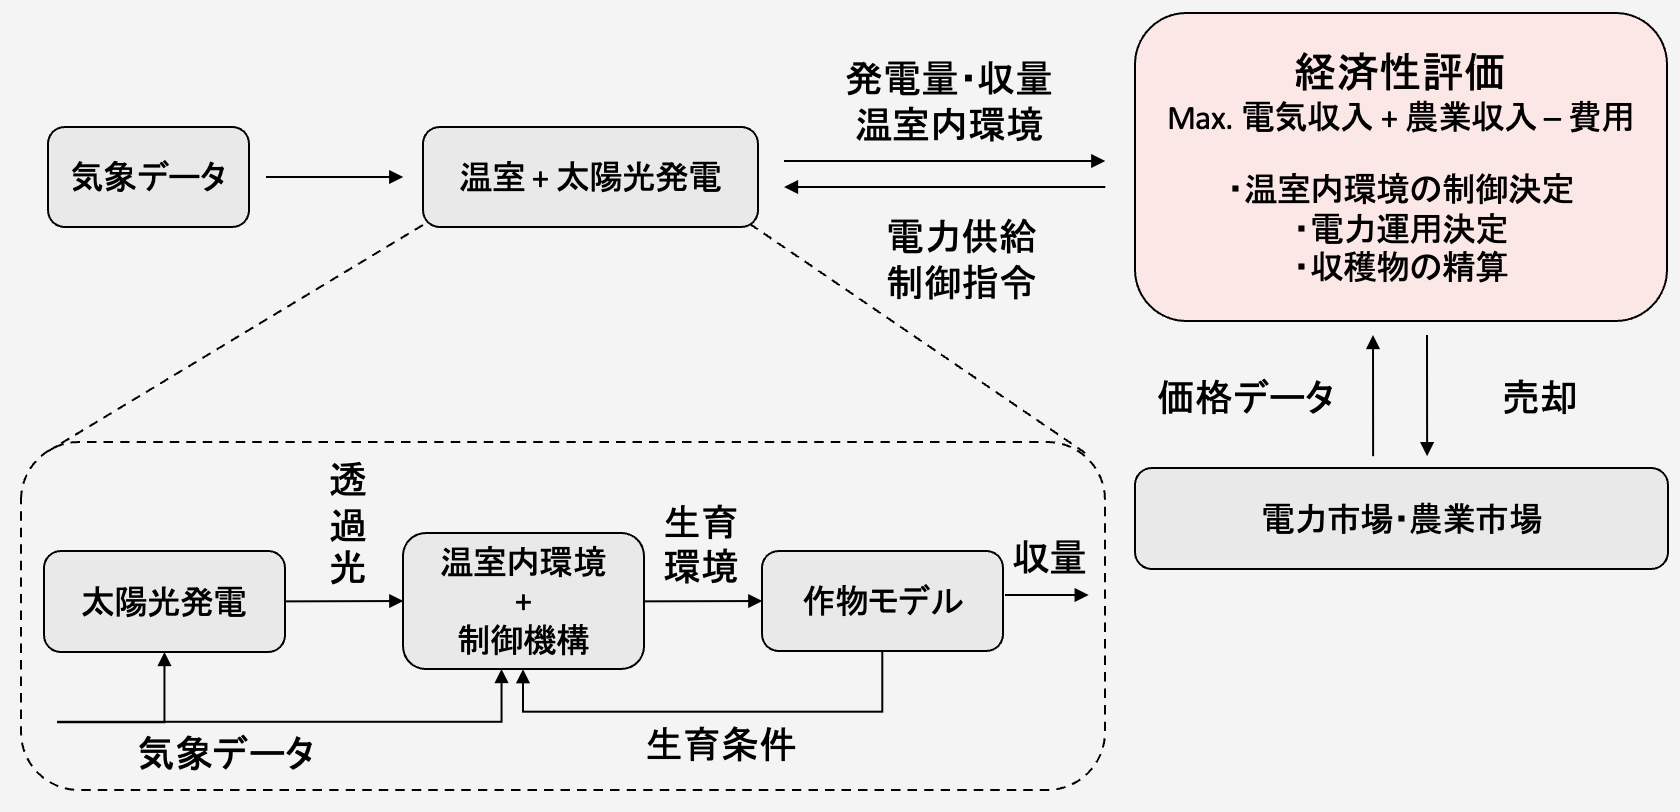
\includegraphics[width=0.9\linewidth]{fig/wholeSystem.png}
    \caption{モデル全体の概要}
    \label{fig:wholeSystem}
\end{figure}

本研究はシミュレーションによる評価を主な手法とし、実証実験については今後の課題とする予定である。

まず、温室に営農型太陽光発電を導入し、その経済性を評価するモデル全体の概要を \fig{wholeSystem} に示す。
シミュレーションの手順は以下に示す通りである。

\begin{enumerate}
    \item 気象データから太陽光発電における発電電力を算出する
    \item 気象データと太陽光パネルを通過する光から温室内の環境を算出する
    \item 温室内の環境を作物の生育条件と照らし合わせ、必要な制御を算出する
    \item 制御に必要な電力については発電電力の使用を考慮し、制御を行う
    \item 制御によって調整された温室内の環境から作物の収量を算出する
    \item 市場の価格データを取得し、発電電力と収穫物の売却により得られる売上を算出する
    \item 売上から費用を差し引き、得られる収益を評価関数として経済性を評価する
    \item 経済性を最大化させるように温室内の環境制御や電力運用、太陽光パネルの設置方法などの改善を図る
\end{enumerate}


\section{温室の設計}
\subsection{温室の設置場所と規格}
シミュレーションを行うにあたって、まずは温室の設置場所と設計を決定した。設置場所は取得可能な気象データの場所から茨城県つくば市とした。

続いて、温室の向きを決定する。北緯30\(^\circ\)から45\(^\circ\)に位置する日本では、東西棟の方が冬季における日射透過率は南北棟よりも10\%前後高いものの、日射が不均一になるという欠点がある。その一方で、南北棟は冬季以外では東西棟の日射透過率を上回り、さらには屋根傾斜角や連棟数がほとんど日射透過率に影響しない。これらの理由から南北棟の温室が多くなっている\cite{Samejima2021}とのことであったのため、本研究でも南北棟を採用することとした。

両屋根型の単棟とし、規格は\tab{housedesign}に示すパラメータを用いた。

\begin{table}[ht]
    \caption{温室の規格}
    \label{tab:housedesign}
    \centering
    \begin{tabular}{lcrrrrc}
        \toprule % --- booktabs: 上の罫線 ---
        項目 & 値\\
        \midrule % --- booktabs: 中間の罫線 ---
        東西方向の長さ & 10 m\\
        南北方向の長さ & 30 m\\
        軒高 & 4 m\\
        屋根傾斜角 & 40 \(^\circ\)\\
        \bottomrule % --- booktabs: 底の罫線 ---
    \end{tabular}
\end{table}


\fig{bifacialPV}はbifacial\_radiance上で設計した、温室に設置されたPV部分の模型であり、南北の屋根側面の三角形部分以外の全ての面に両面PVを設置することとした。

\begin{figure}[ht]
    \centering
    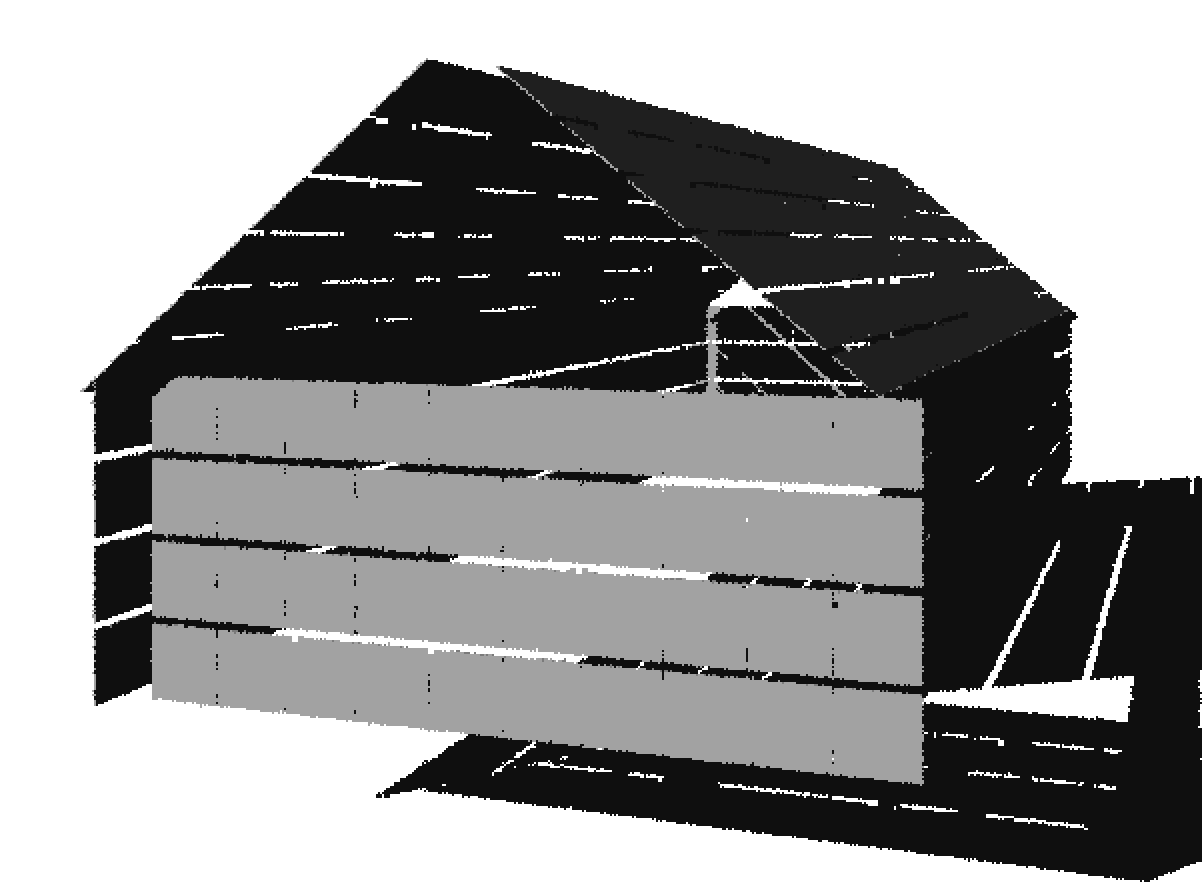
\includegraphics[width=0.7\linewidth]{fig/PVmodel.png}
    \caption{温室に設置された両面PV}
    \label{fig:bifacialPV}
\end{figure}

\subsection{温室内外の設備}
あいうえお

\section{シミュレーションモデル}
\subsection{シミュレーション環境}
気象データから太陽光パネルが受ける日射量を算出する部分では、NRELが提供するbifacial\_radianceを用いている。bifacial\_radianceは、レイトレーシングによって両面PVシステムのパフォーマンスのシミュレーションを行うことができるpythonのパッケージである\cite{Bifacialradiance}。

温室内の環境と必要な制御を算出する部分では、MathWorksが提供するMATLAB Simulinkを用いている\cite{MATLAB}。視覚的なブロック線図によりシミュレーションの構造の把握が比較的容易となる。\fig{Simulink}は現時点で構成されているモデルの全体像である。

\begin{figure}[ht]
    \centering
    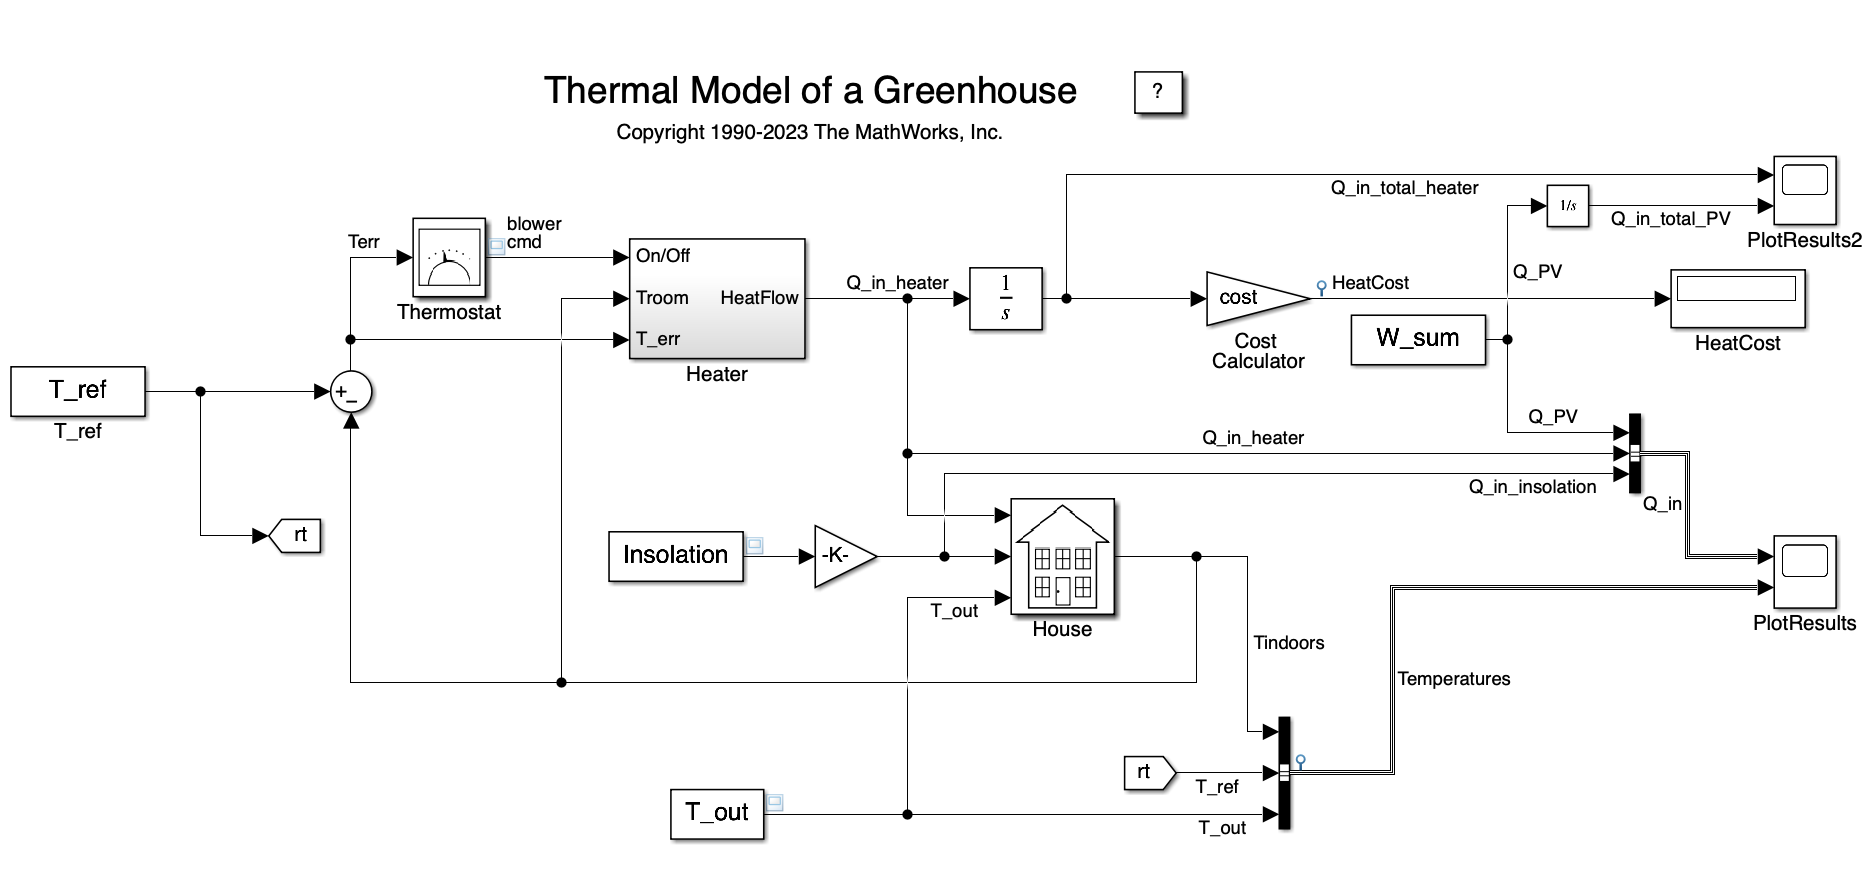
\includegraphics[width=0.9\linewidth]{fig/Simulink.png}
    \caption{Simulinkモデルの全体像}
    \label{fig:Simulink}
\end{figure}


\subsection{太陽光発電の発電電力}
太陽光発電の発電電力\(P_{\text{PV}}\)は、bifacial\_radianceによって求められた太陽光パネルに当たる日射量に一定の発電効率\(\eta\)を乗算することで求めた。
太陽光パネルの各面に当たる日射強度と各面の面積を、
\begin{itemize}
    \item \(I_{\text{ER}}, S_{\text{ER}}\): 東側の屋根に対する日射強度と面積
    \item \(I_{\text{WR}}, S_{\text{WR}}\): 西側の屋根に対する日射強度と面積
    \item \(I_{\text{EW}}, S_{\text{EW}}\): 東側の壁に対する日射強度と面積
    \item \(I_{\text{WW}}, S_{\text{WW}}\): 西側の壁に対する日射強度と面積
    \item \(I_{\text{SW}}, S_{\text{SW}}\): 南側の壁に対する日射強度と面積
    \item \(I_{\text{NW}}, S_{\text{NW}}\): 北側の壁に対する日射強度と面積
\end{itemize}
とすると、全体の発電電力は式\eqref{Ppv}で表される。

\begin{align}
    P_{\text{PV}} =  (I_{\text{ER}} S_{\text{ER}} + I_{\text{WR}} S_{\text{WR}} + I_{\text{EW}} S_{\text{EW}} + I_{\text{WW}} S_{\text{WW}} + I_{\text{SW}} S_{\text{SW}} + I_{\text{NW}} S_{\text{NW}}) \cdot \eta
    \label{Ppv}
\end{align}


\subsection{温室内の温度}
温室内の温度は、
\begin{itemize}
    \item \(Q_\text{flow}\): 熱貫流による熱エネルギーの出入り
    \item \(Q_\text{heater}\): ヒーターによる熱エネルギーの供給
    \item \(Q_\text{insolation}\): 照射する日光による熱エネルギーの供給
\end{itemize}
によって変化するものとし、温室内に供給される熱を正として扱う。

まず、熱貫流による熱エネルギーの出入りは、室外の気温\(T_\text{out}\)、室内の気温\(T_\text{in}\)、熱貫流率\(U\)、温室の表面積\(S\)から式\eqref{Qflow}で表される。
\begin{align}
    Q_\text{flow} = (T_\text{out} - T_\text{in}) \cdot U \cdot S
    \label{Qflow}
\end{align}

ヒーターによる熱エネルギーの供給は、ヒーターが1秒あたりに放出する空気量\(Mdot\)、ヒーターが放出する空気の温度\(T_\text{heater}\)、空気比熱\(c\)から式\eqref{Qheater}で表される。

\begin{align}
    Q_\text{heater} = (T_\text{heater} - T_\text{in}) \cdot Mdot \cdot c
    \label{Qheater}
\end{align}

日射による熱エネルギーの供給は、温室の底面積\(S_\text{bottom}\)、日射強度\(I_\text{bottom}\)、温室の遮蔽係数\(G\)、温室内での太陽エネルギーの吸収率\(\mu\)から式\eqref{Qinsolation}で表される。

\begin{align}
    Q_\text{insolation} = I_\text{bottom} \cdot S_\text{bottom} \cdot G \cdot \mu
    \label{Qinsolation}
\end{align}

以上から温室内の温度変化\(\Delta T\)は、温室内の空気の質量\(M\)と空気比熱\(c\)から式\eqref{DeltaT}で表される。ただし、空気の質量\(M\)は、空気の密度を\(D_\text{air}\)、温室の体積を\(V\)とすると、\(M = D_\text{air} \cdot V\)である。

\begin{align}
    \Delta T = (Q_\text{flow} + Q_\text{heater} + Q_\text{insolation}) \cdot M \cdot c
    \label{DeltaT}
\end{align}

シミュレーションでは、ヒーターの出力を調整することで、温室内の温度が対象作物の生育条件に適した温度となるようにする。


\section{作物の生育条件}
本研究ではイチゴの施設栽培を例にとり、シミュレーションを行うこととした。岐阜県農業技術センターの研究報告\cite{strawberry2010}によると、イチゴを温室で栽培する際に昼間は28 \(^\circ\)Cとし、夜間は最低温度を5 \(^\circ\)Cとすると省エネルギーな栽培となるという結果が得られていたため、本研究も同じ温度設定を採用し、簡易的に温室内の温度を6時から18時を28 \(^\circ\)C、18時から6時を5 \(^\circ\)Cと設定した。

\chapter{結果}
以下に示すのは、茨城県つくば市においてイチゴの施設栽培を行う際の、2023年12月1日分のシミュレーション結果である。


\fig{QinTemp}の下のグラフは、温室内の温度\(T_\text{in}\)と室外の温度\(T_\text{out}\)、さらにイチゴの生育条件に合わせて設定した温度\(T_\text{ref}\)を表示したものである。一方、上のグラフは、ヒーターによって供給された熱量\(Q_\text{heater}\)と日射によって供給された熱量 \(Q_\text{insolation}\)、さらに太陽光発電の発電電力\(P_\text{PV}\)を電気-熱間の変換効率を1として熱量に変換した値を表示したものである。
グラフから設計したヒーターの制御モデルによって温室内の温度を概ね指令値通りに制御できていることが確かめられた。さらに日射による熱エネルギーの供給がある時間帯はヒーターによる熱供給が小さくなっていることがわかる。


\begin{figure}[ht]
    \centering
    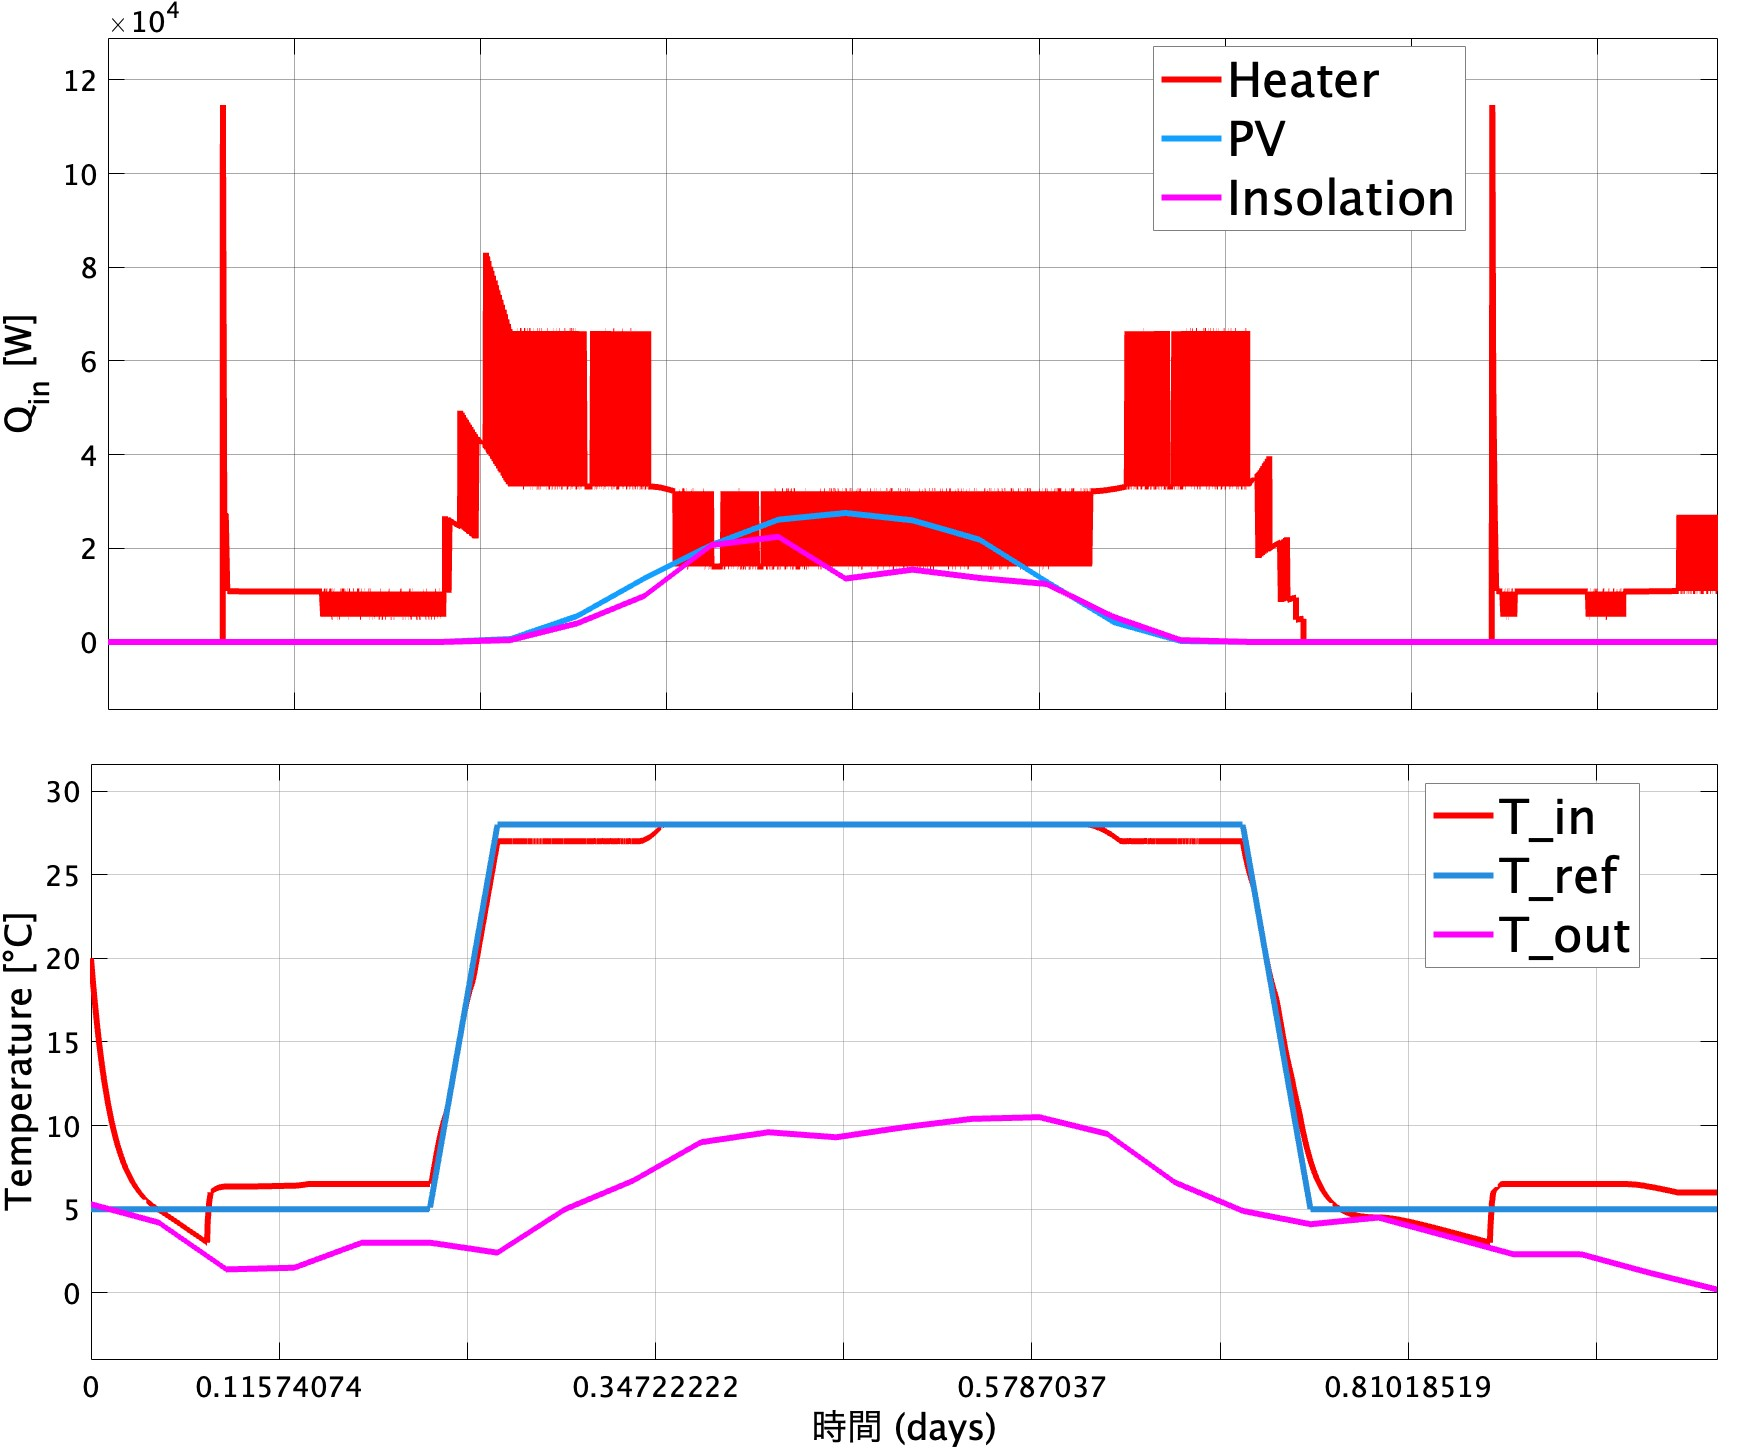
\includegraphics[width=0.7\linewidth]{fig/Qin-Temp.jpg}
    \caption{1日の温度と熱量}
    \label{fig:QinTemp}
\end{figure}


\fig{QinTotal}は、ヒーターによって供給された熱量と発電電力を電気-熱間の変換効率を1として熱量に変換した値を累積させた結果を示したものである。
単純な1日の累積ではヒーターによって供給された熱量の方が3倍程度大きいという結果が得られた。しかし、実際に電気を熱に変換する場合、ヒートポンプやエアコンのCOPは1を超えることが多いため、発電された電力の自家消費によって温室での電力需要を賄うことができる可能性は高い。後藤らによる研究\cite{Cop2013}では、温室におけるヒートポンプのCOPは定格条件下で平均5程度、冬季夜間の運転で平均3程度のCOPという結果が得られていた。さらにこのCOPの値は2013年時点でのものであるため、2024年現在ではさらに高いCOPとなることが期待できる。

\begin{figure}[ht]
    \centering
    \includegraphics[width=0.8\linewidth]{fig/Qintotal.jpg}
    \caption{1日の累積の熱量}
    \label{fig:QinTotal}
\end{figure}


\chapter{結論}
\section{現時点での成果}
現時点では、農業と発電事業を統合したシステムの経済性を評価するためのシミュレーションの実施において、温室に太陽光パネルを設置したモデルの全体像を構築し、経済性を評価するための方法を定めた上で、シミュレーションの基礎的な部分の設計と実行および結果の取得が完了している。上記に示した結果から、温室の電力需要を発電電力の自家消費で賄うことができる可能性が示され、それに付随する経済性の向上と環境負荷低減の可能性についても示すことができた。しかし、現時点の結果は全体像の一部に過ぎず、より詳細な研究が必要である。

\section{今後の課題}
以上を踏まえ、今後の課題として次のようなものが考えられる。
\begin{itemize}
    \item シミュレーション期間の拡大: 現時点では2023年12月1日分の結果のみがまとめられている。気象条件は月日によって大きく変動するため、経済性の評価を行うためには少なくともイチゴの生育期間分のシミュレーションが必要である。
    \item 温室内環境の制御機構の拡張: 現時点ではヒーターでの加温のみを考慮しているが、実際の栽培により近づけるためには土を温める仕組みや日照時間を補填するための電灯についても考慮に入れ、作物の生育条件を満たす環境を整備する必要がある。
    \item レイトレーシングの精度向上: 現時点では簡易的な太陽光パネルの設置のみでレイトレーシングを行い日射強度を算出しているが、実際は作物や温室内の設備が存在することによる影響があるため、より精密なシミュレーションのためには、詳細な環境を組み込む必要がある。
    \item 発電電力の運用方法の検討: 現時点では発電電力の具体的な運用方法については検討できていないが、経済性の評価に至るには瞬時的な自家消費や売電、さらには蓄熱・蓄電を考慮した運用モデルを決定することが必要となる。
\end{itemize}

\chapter{メモ}
\begin{itemize}
    \item 最大暖房負荷\(Q_\text{h}\): 外気温が最も低下し、晴天で放射冷却が大きい場合に必要な暖房熱量\cite{Samejima2021}。
    \begin{itemize}
        \item \(Q_\text{h} = A_\text{s} (T_\text{i} - T_\text{o}) U_\text{0} (1 - f_\text{r}) f_\text{w}\)
        \item \(A_\text{s}\): 温室の表面積(m\(^2\))
        \item \(T_\text{i}\): 室内気温(\(^\circ \text{C}\))
        \item \(T_\text{o}\): 外気温(\(^\circ \text{C}\))
        \item \(U_\text{0}\): 一重被覆における暖房負荷係数(熱貫流, 換気伝熱, 地中伝熱を含んだ係数で、ガラス温室の場合6.2、塩化ビニル温室の場合6.6 W\(\cdot\)m\(^{-2}\cdot ^\circ \text{C}^{-1}\)
        \item \(f_\text{r}\): 保温被覆を行う場合の熱節減率
        \item \(f_\text{w}\): 風速の補正係数(通常は1.0,  強風地域では1.1)
        \item 暖房負荷は容積ではなく表面積に比例する
    \end{itemize}
\end{itemize}

\backmatter

\bibliographystyle{tipsj.bst}
\bibliography{ref.bib}

% \chapter{発表文献}

% \section*{学術論文誌}

% \section*{学会発表}

% \chapter{謝辞}

% 調整力に関する研究が行われている\cite{Cai2022,Ehara2023}。
% \fig{figure_name}と\fig{subfigure_name}に図の例を示す。
% \eq{kaya}に茅恒等式を示す。
% \tab{si}にSI組立単位を示す。

% \begin{figure}[t]
%     \centering
%     \subfigure[Subfigure name 1.]{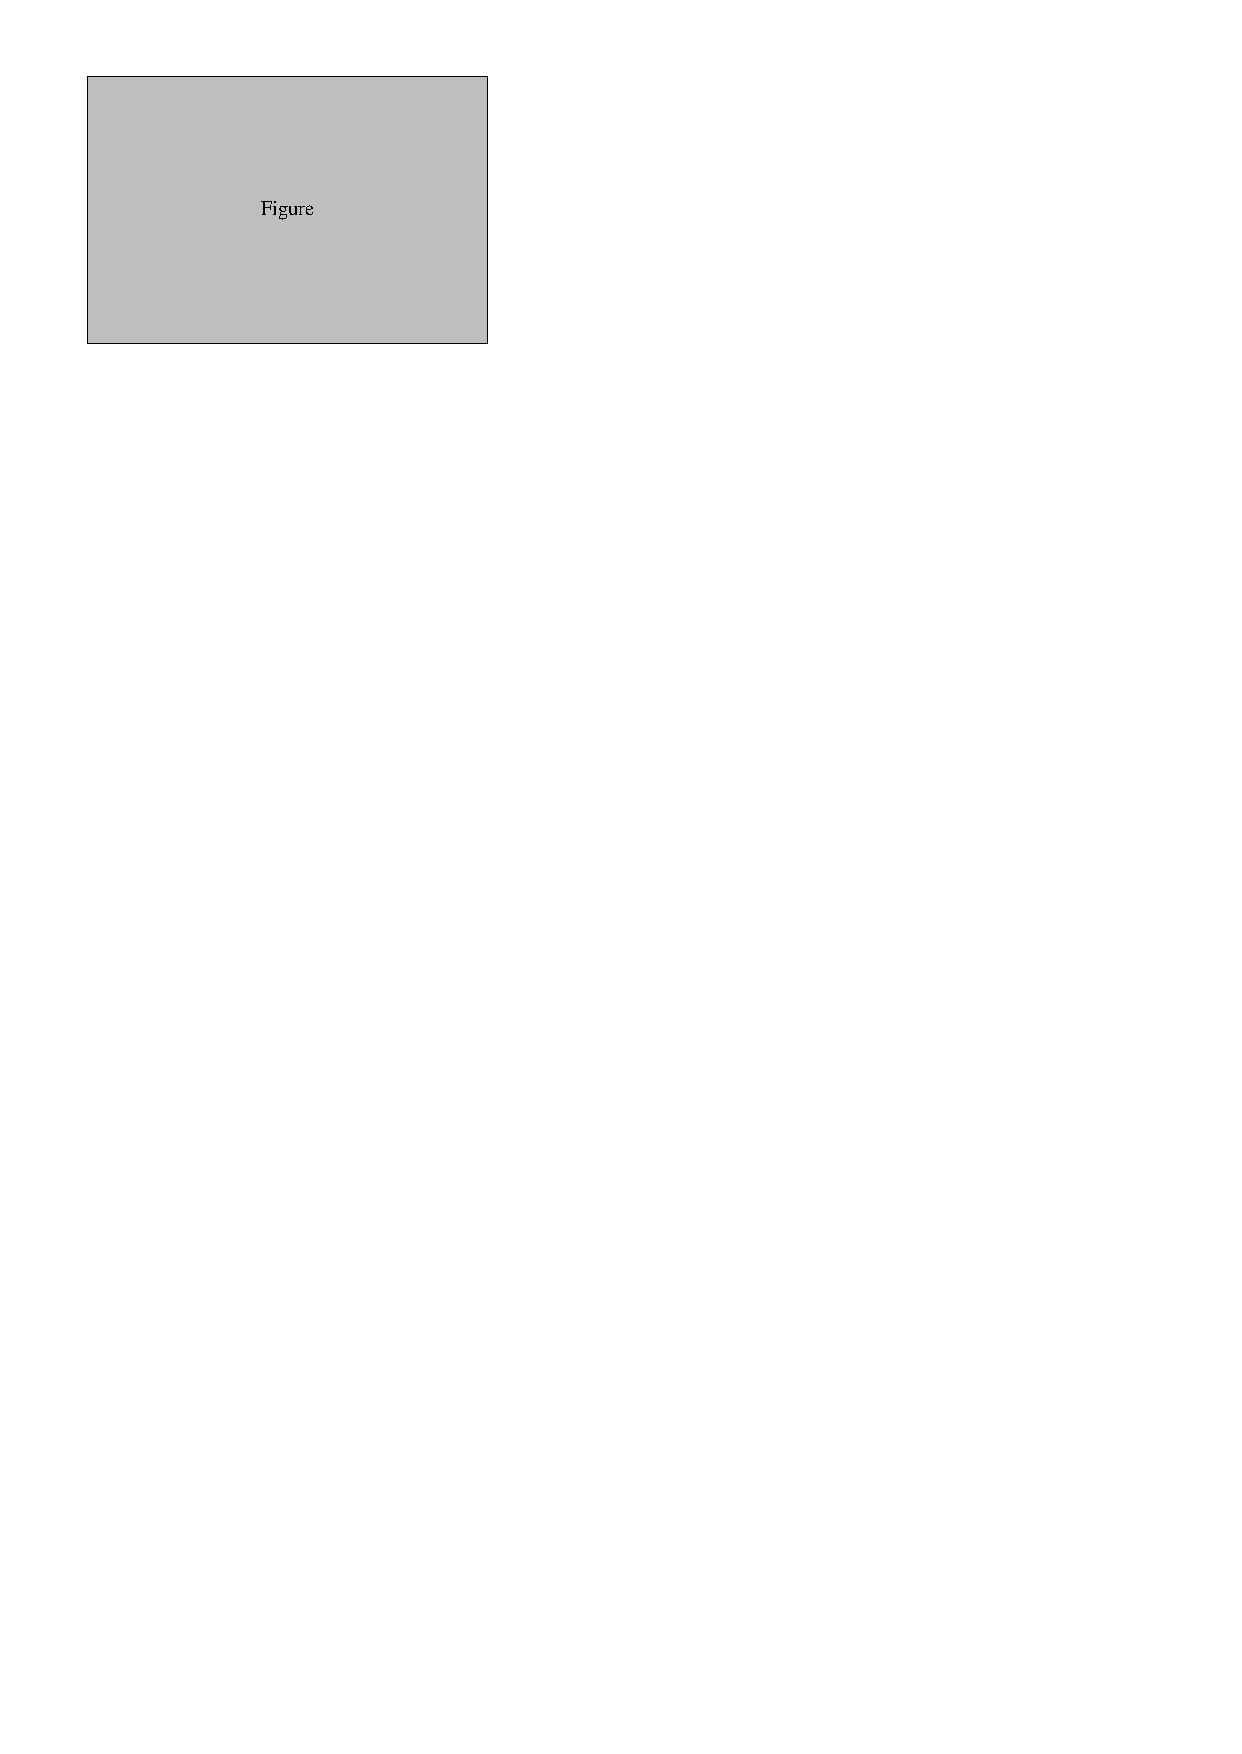
\includegraphics[width=0.45\linewidth]{sample.pdf}\label{fig:subfigure_name_1}}
%     \subfigure[Subfigure name 2.]{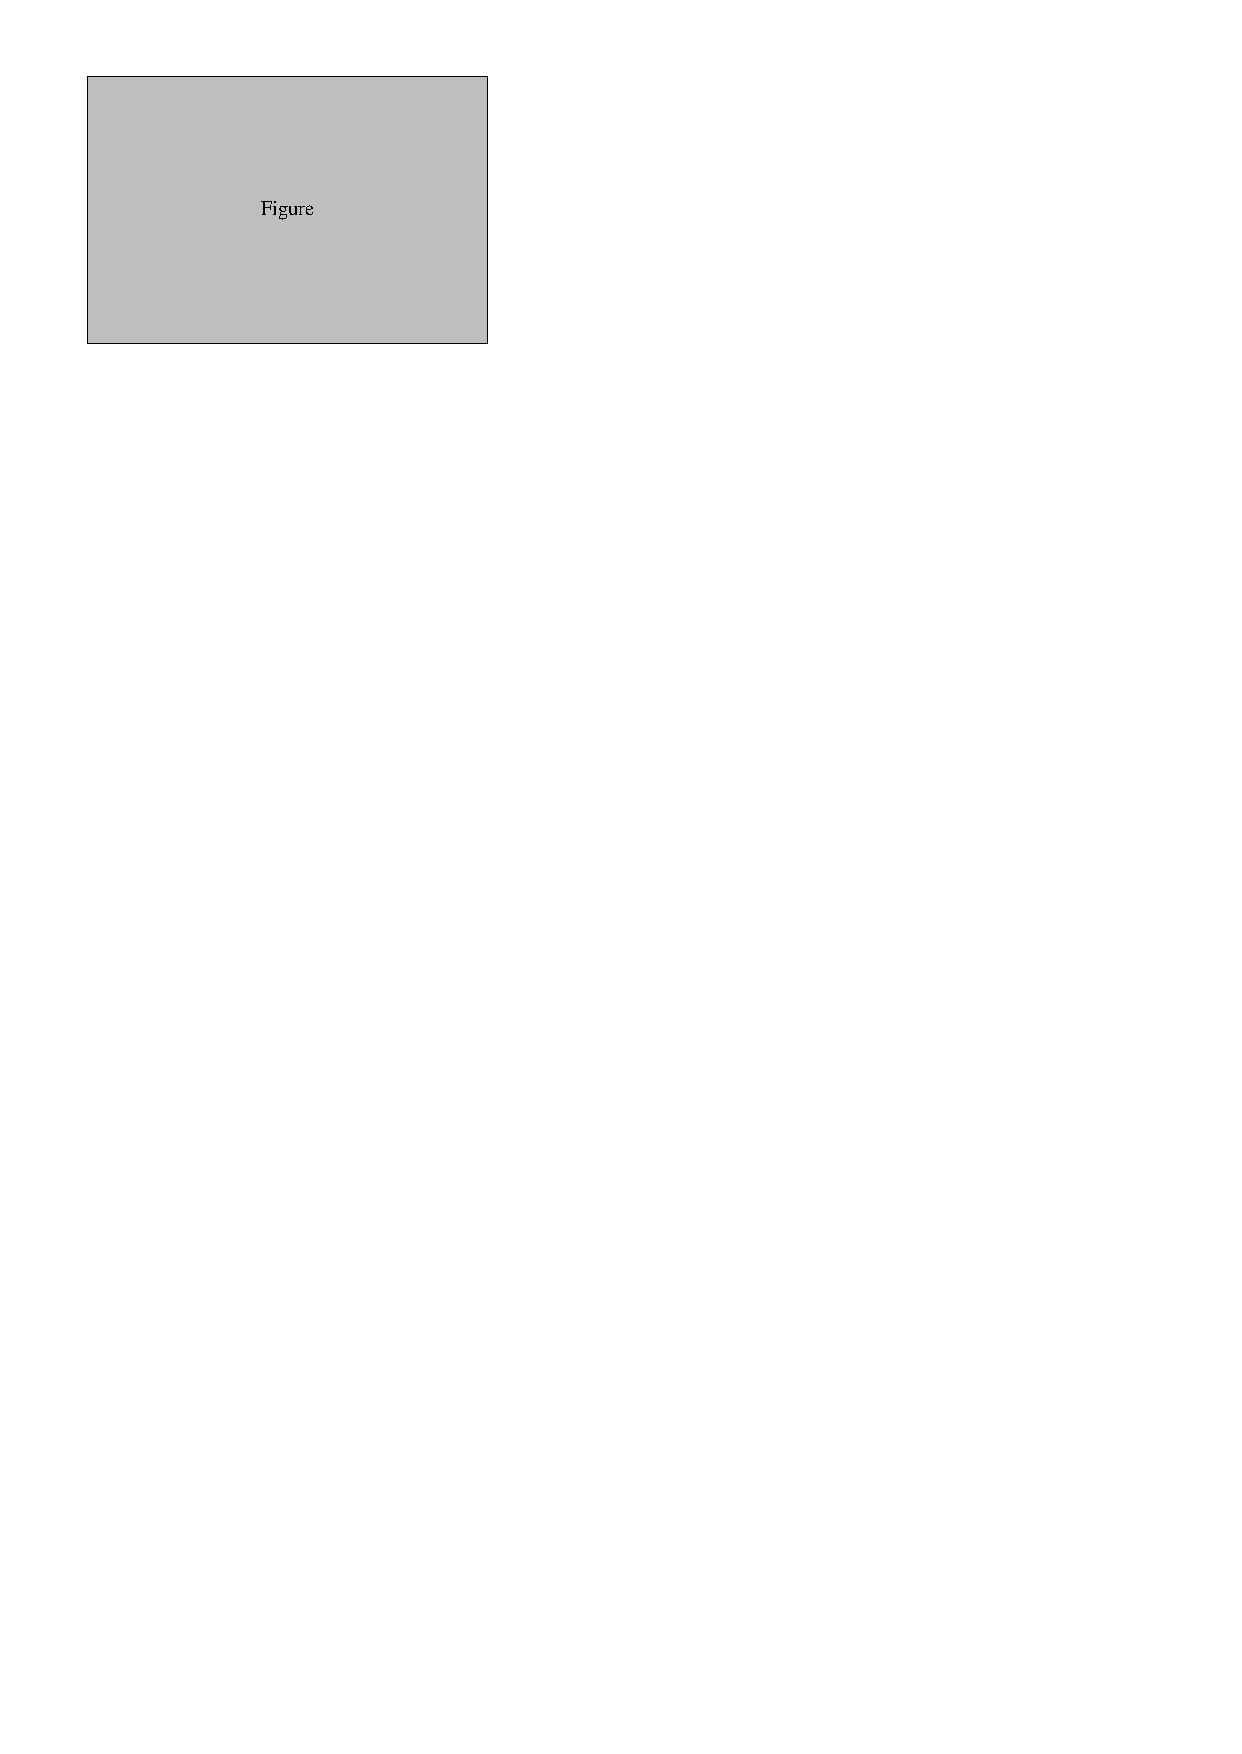
\includegraphics[width=0.45\linewidth]{sample.pdf}\label{fig:subfigure_name_2}}
%     \caption{Subfigure name.}
%     \label{fig:subfigure_name}
% \end{figure}

% \begin{table}[t]
% \caption{SI組立単位}
% \label{tab:si}
% \centering
%   \begin{tabular}{lcrrrrc}
%     \toprule % --- booktabs: 上の罫線 ---
%     物理量 & 単位 & \multicolumn{4}{c}{SI単位系の基本単位} & 他の単位 \\
%     \cmidrule(lr){3-6} % --- booktabs: 3 から 9 列の罫線 ---
%     & 記号 & m & kg & s & A\\
%     \midrule % --- booktabs: 中間の罫線 ---
%     力 & N & 1 & 1 & -2 & & \\
%     エネルギー & J & 2 & 1 & -2 &  &N$\cdot$m \\
%     仕事率 & W & 2 & 1 & -3 &  &J$\cdot$s$^{-1}$ \\
%     \addlinespace[5mm] % --- booktabs: 行間スペース ---
%     電圧 & V & 2 & 1 & -3 & -1 &W$\cdot$A$^{-1}$ \\
%     磁束 & Wb & 2 & 1 & -2 & -1 &  V$\cdot$s \\
%     \bottomrule % --- booktabs: 底の罫線 ---
%   \end{tabular}
% \end{table}

\end{document}
